\documentclass[11pt, oneside]{article}
\usepackage[margin=.9in]{geometry}
\usepackage{pgfplots}
\pgfplotsset{compat=default}
\newcommand{\cuckoo}{{\rm cuckoo}}
\newcommand{\hash}{{\rm siphash}}
\usepackage{hyperref}
\usepackage{listings}
\title{Cuckoo Cycle: \protect\\ a memory-hard proof-of-work system}
\author{John Tromp}
\begin{document}
\maketitle

\begin{abstract}
We introduce the first trivially verifiable, scalable and
tmto\footnote{time-memory trade-off}-hard proof-of-work system.
\end{abstract}

\section{Introduction}
A ``proof of work'' (PoW) system allows a verifier to check with negligible
effort that a prover has expended a large amount of computational effort.
Originally introduced as a spam fighting measure, 
where the effort is the price paid by an email sender for demanding the
recipient's attention, they now form one of the cornerstones of
crypto-currencies.

As proof-of-work for new blocks of transactions,
Bitcoin~\cite{nakamoto2009bitcoin} uses hashcash~\cite{back2002}.
This requires finding a nonce value such that
twofold application of the cryptographic hash function SHA256
to this nonce (and the rest of the block header) results in a number with
many leading 0s. The bitcoin protocol dynamically adjust this ``difficulty''
number so as to maintain a 10-minute average block interval. Starting out at
32 leading zeroes in 2009, the number has steadily climbed and is currently
at 64, representing an incredible $2^{64}/10$ double-hashes per minute.
This growth was enabled by the migration of hash computation from 
desktop processors (CPUs) to graphics-card procecssors (GPUs),
to field-programmable gate arrays (FPGAs), and finally to custom designed
chips (ASICs).

Downsides of this development include high investment costs, rapid
obsolesence, centralization of mining power, and large power consumption.
Although ASICs are the most energy-efficient way of computing hashes,
the tiny amount of die-space needed for a single SHA256 circuit allows
a huge number of them (e.g. 1440 on KnC's Neptune) to be crammed onto a
single chip, consuming 100s of Watts and requiring ample cooling.
Thus, energy costs dominate the economics of mining.

This has led people to look for alternative proof-of-work systems
that, by requiring a nontrivial amount of memory, resist such
massive parallelizability, and narrow the performance gap
with commodity hardware. Memory chips, in the form of DRAM,
have only a tiny portion of their circuitry active at any time,
and thus require orders of magnitude less power.

Litecoin replaces the SHA256 hash function in hashcash by a single round
version of the {\em scrypt} key derivation function. Its memory requirement
of 128KB is a compromise between computation-hardness for the prover and
verification efficiency for the verifier. Although designed to be
GPU-resistant, GPUs are now at least an order of magnitude faster
than CPUs for Litecoin mining. ASICs first appeared on the market in early 2014 and are expected to dominate Litecoin mining by the fourth quarter.

Primecoin~\cite{king2013} is an interesting design based on finding long
Cunningham chains of prime numbers, using a two-step process of filtering
candidates by {\em sieving}, and applying pseudo-primality tests to remaining
candidates. The most efficient implementations are still CPU based.
Downsides to this proof-of-work are its complexity and the scope for
algorithmic improvements that may be kept private. Its memory requirements,
while larger than Litecoin's, are still modest.

Momentum~\cite{larimer2013} proposes finding birthday collisions of hash
outputs as proof-of-work, the simplest way to combine scalable memory usage
with trivial verifiability. Its memory requirements are not very strict
though. as Bloom filters or rainbow tables can identify collisions, and
parallellizes well.

Adam Back~\cite{back2014} has a good overview of proof-of-work papers past
and present.

\section{Memory latency; the great equalizer}
While cpu-speed and (sequential) memory bandwidth are highly variable across
time and architectures, main memory latencies have remained relatively
stable. This suggests making the proof-of-work system latency-bound to level
the mining playing field.
Ideally, it should have the following properties:
\begin{description}
\item[verify-trivial] A proof can be checked in microseconds rather than
 milliseconds.
\item[scalable] The amount of memory needed is a parameter that can scale
  arbitrarily.
\item[linear] Amount of computational steps and memory accesses
  are linear in the amount of memory.
\item[tmto-hard] Using only half as much memory should incur several orders
  of magnitude slowdown.
\item[random-access] RAM is accessed randomly, making
  sequential bandwidth and caches mostly irrelevant.
\item[parallel-hard] The algorithm cannot be parallellized within
  a single instance, i.e. proof attempt).
\item[simple] The algorithm should be sufficiently simple that one can be
  convinced of its optimality.
\end{description}
Combined, these properties ensure that a proof-of-work system is entirely
constrained by main memory latency and scales appropriately for any
application.

We introduce the very first proof-of-work system that is both verify-trivial
and tmto-hard. Furthermore, it satisfies all other properties,
except for parallel-hardness (see the later section on parallelizability).
Amazingly, it amounts to little more than enumerating nonces and storing them
in a hashtable. While all hashtables break down when trying to store more
items than it was designed to handle, in one hashtable design in particular
this breakdown is of a special nature that can be turned into a concise and
easily verified proof. Enter the cuckoo hashtable.

\section{Cuckoo hashing}
Introduced by Rasmus Pagh and Flemming Friche
Rodler~\cite{Pagh04cuckoohashing}, a cuckoo hashtable consists of two
same-sized tables each with its own hash function mapping a key to a table
location, providing two possible locations for each key.
Upon insertion of a new key, if both locations are already occupied by keys,
then one is kicked out and inserted in its alternate location, possibly
displacing yet another key, repeating the process until either a vacant
location is found, or some maximum number of iterations is reached.
The latter can only happen once cycles have formed in the {\em Cuckoo graph}.
This is a bipartite graph with a node for each location and an
edge for every key, connecting the two locations it can reside at.
This naturally suggests a proof-of-work problem, which we now formally
define.

\section{The proof-of-work function}
Fix an (even) number of nodes $8 \leq N < 2^{32}$, a number of edges $N/4 < E
\leq N$, and an (even) cycle length $4 \leq L < 256$.
Function $\cuckoo$ maps any 128-bit key $k$ (the header digest) to a
bipartite graph $G = (V_0 \cup V_1, E)$, where $V_0$ is the set of integers
modulo $N_0=N/2+1$, $V_1$ is the set of integers modulo $N_1=N/2-1$, and $E$
has an edge between $\hash(k,n) \bmod N_0$ in $V_0$ and $\hash(k,n) \bmod
N_1$ in $V_1$ for every nonce $0 \leq n < E$. A proof for $G$ is a subset of
$L$ nonces whose corresponding edges form an $L$-cycle in $G$.

\section{Solving the proof-of-work problem}
We enumerate the $E$ nonces, but instead of storing the nonce itself as a key
in the Cuckoo hashtable, we store the alternate key location at the key
location, and forget about the nonce.  We thus maintain the {\em directed}
cuckoo graph, in which the edge for a key is directed from the location where
it resides to its alternate location.  Moving a key to its alternate location
thus corresponds to reversing its edge.  The outdegree of every node in this
graph is either 0 or 1.  When there are no cycles yet, the graph is a {\em
forest}, a disjoint union of trees.  In each tree, all edges are directed,
directly, or indirectly, to its {\em root}, the only node in the tree with
outdegree 0.  Initially there are just $N$ singleton trees consisting of
individual nodes which are all roots.
Addition of a new key causes a cycle if and only if its two endpoints are
nodes in the same tree, which we can test by following the path from each
endpoint to its root.
In case of different roots, we reverse all edges on the shorter of the two
paths, and finally create the edge for the new key itself, thereby joining
the two trees into one.
The left diagram below shows the directed cuckoo graph for header `header' on
$N=9+7$ nodes after adding edges
$(3,16),(5,15),(6,16),(7,16),(5,10),(6,13),(6,12),(9,14)$ and $(4,14)$ (nodes
with no incident edges are omitted for clarity).
In order to add the 10th edge $(7,10)$, we follow the paths $7 \rightarrow 16
\rightarrow 3$ and $10 \rightarrow 5$ to find different roots $3$ and $5$.
Since the latter path is shorter, we reverse it to $5 \rightarrow 10$ so we
can add the new edge as $(10 \rightarrow 7)$, resulting in the right diagram.
\begin{center}
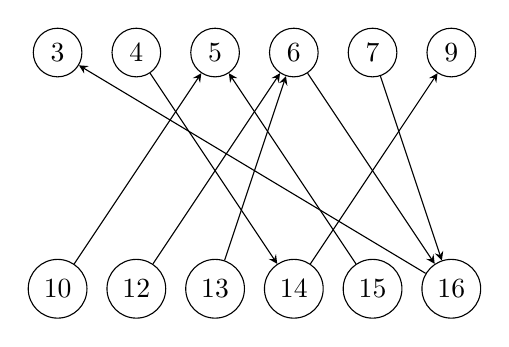
\begin{tikzpicture}[>=stealth]
\node  (3) at (1, 2) [shape=circle,draw] {3};
\node  (4) at (2, 2) [shape=circle,draw] {4};
\node  (5) at (3, 2) [shape=circle,draw] {5};
\node  (6) at (4, 2) [shape=circle,draw] {6};
\node  (7) at (5, 2) [shape=circle,draw] {7};
\node  (9) at (6, 2) [shape=circle,draw] {9};
\node (10) at (1,-1) [shape=circle,draw] {10};
\node (12) at (2,-1) [shape=circle,draw] {12};
\node (13) at (3,-1) [shape=circle,draw] {13};
\node (14) at (4,-1) [shape=circle,draw] {14};
\node (15) at (5,-1) [shape=circle,draw] {15};
\node (16) at (6,-1) [shape=circle,draw] {16};
\draw [->] (16) -- (3);
\draw [->] (15) -- (5);
\draw [->]  (6) -- (16);
\draw [->]  (7) -- (16);
\draw [->] (10) -- (5);
\draw [->] (13) -- (6);
\draw [->] (12) -- (6);
\draw [->] (14) -- (9);
\draw [->]  (4) -- (14);
\end{tikzpicture}\hspace{3cm}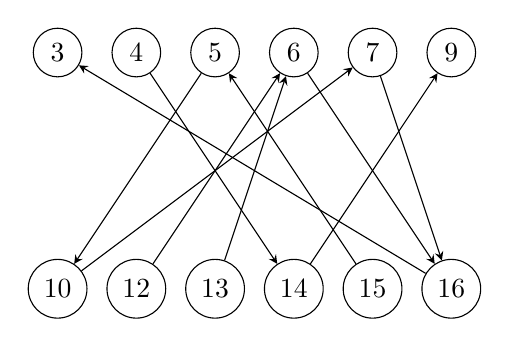
\begin{tikzpicture}[>=stealth]
\node  (3) at (1, 2) [shape=circle,draw] {3};
\node  (4) at (2, 2) [shape=circle,draw] {4};
\node  (5) at (3, 2) [shape=circle,draw] {5};
\node  (6) at (4, 2) [shape=circle,draw] {6};
\node  (7) at (5, 2) [shape=circle,draw] {7};
\node  (9) at (6, 2) [shape=circle,draw] {9};
\node (10) at (1,-1) [shape=circle,draw] {10};
\node (12) at (2,-1) [shape=circle,draw] {12};
\node (13) at (3,-1) [shape=circle,draw] {13};
\node (14) at (4,-1) [shape=circle,draw] {14};
\node (15) at (5,-1) [shape=circle,draw] {15};
\node (16) at (6,-1) [shape=circle,draw] {16};
\draw [->] (16) -- (3);
\draw [->] (15) -- (5);
\draw [->]  (6) -- (16);
\draw [->]  (7) -- (16);
\draw [->]  (5) -- (10);
\draw [->] (13) -- (6);
\draw [->] (12) -- (6);
\draw [->] (14) -- (9);
\draw [->]  (4) -- (14);
\draw [->] (10) -- (7);
\end{tikzpicture}
\end{center}
When adding the 11th edge $(3,15)$, we find the singleton path $3$ and the
path $15 \rightarrow 5 \rightarrow 10 \rightarrow 7 \rightarrow 16
\rightarrow 3$ with equal roots.
In this case, we can compute the length of the resulting cycle as
1 plus the sum of the path-lengths to the node where the two paths first join.
In the diagram, the paths first join at the root, and the cycle length is computed as $1+0+5=6$.
If the cycle length equals $L$, then we solved the problem, and recover the proof
by enumerating nonces once more and checking which ones formed the cycle.
If not, then we keep the graph acyclic by ignoring the edge.
There is some probability of overlooking other $L$-cycles
through that edge, but in the important case of having few cycles
in the cuckoo graph to begin with, it hardly affects the rate of solution finding.

\section{Union-find}
The above representation of the directed cuckoo graph is an example of
a {\em disjoint-set data structure}~\cite{wikidsds2014}, and our algorithm is
closely related to the well known union-find algorithm, where the find operation
determines which subset an element is in, and the union operation joins two subsets
into a single one. For each edge addition to the cuckoo graph we perforn the equivalent
of two find operaations and one union operation.
The difference is that the union-find algorithm is free to add
directed edges between arbitrary elements. Thus it can join two subsets by adding an edge
from one root to another, with no need to reverse any edges. Conversely, our algorithm
can be seen as the first one that solves the union-find problem by maintaining
a direction on all union operations while keeping the maximum outdegree at 1.

\section{Implementation and performance}
The C-program listed in the Appendix is also available online at
\url{https://github.com/tromp/cuckoo} together with a Makefile,
proof verifier and the latest version of this paper. `make test' tests everything.
`make example' reproduces the example shown above.
The main program uses 32 bits per node to represent the directed cuckoo graph,
plus about 56KB per thread for 3 auxiliary arrays.
The {\tt us} and {\tt vs} arrays not only record traversed paths,
but also double as a mini cuckoo table used for storing edges of a solution cycle,
allowing easy recovery of the proof nonces.
The {\tt uvpre} array precomputes edges in blocks of 1024, which was found (inexplicably)
to save up to 30\% runtime.
The left plot below shows both the total runtime in seconds and the runtime of just
the hash computation, as a function of (log)size. The latter is purely
linear, while the former is superlinear due to increasing memory latency
as the nodes no longer fit in cache. The right plot show this more clearly
as the percentage of hashing to total runtime, ending up around 5\%.

\begin{center}
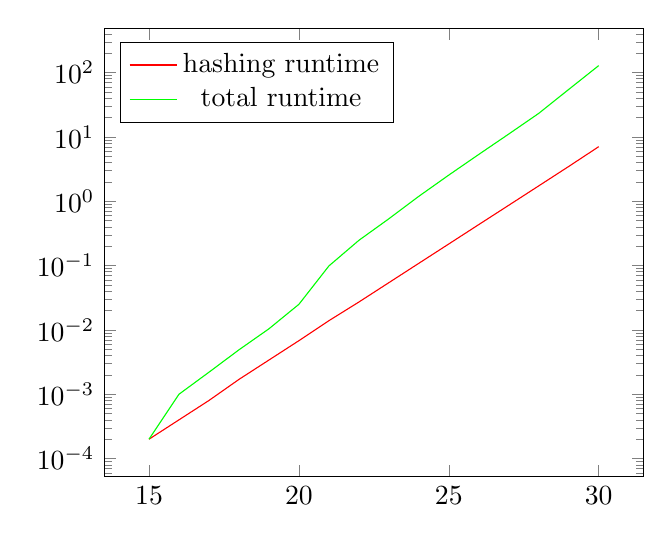
\begin{tikzpicture}
\begin{axis}[ymode=log, legend pos=north west]
\addplot[color=red] coordinates {
% (10,0.0000) (11,0.0000) (12,0.0000) (13,0.0001) (14,0.0001)
(15,0.0002) (16,0.0004) (17,0.0008) (18,0.0017) (19,0.0034)
(20,0.0068) (21,0.0139) (22,0.0271) (23,0.0542) (24,0.1084)
(25,0.2166) (26,0.4336) (27,0.8658) (28,1.7322) (29,3.4719)
(30,7.0389) };
\addlegendentry{hashing runtime}
\addplot[color=green] coordinates {
% (10,0.0000) (11,0.0000) (12,0.0001) (13,0.0001) (14,0.0003)
(15,0.0002) (16,0.0010) (17,0.0022) (18,0.0049) (19,0.0104)
(20,0.0250) (21,0.0986) (22,0.2465) (23,0.5332) (24,1.1922)
(25,2.5505) (26,5.3394) (27,11.0793) (28,23.1984) (29,54.6811)
(30,128.1682) };
\addlegendentry{total runtime}
\end{axis}
\end{tikzpicture}
\hspace{1cm}
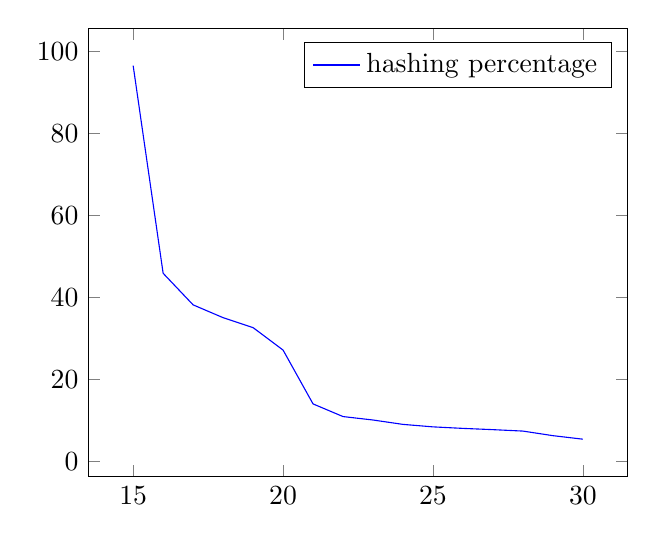
\begin{tikzpicture}
\begin{axis}[legend pos=north east]
\addplot[color=blue] coordinates {
% (10,38.8889) (11,33.3333) (12,45.1613) (13,39.8496) (14,44.6154)
(15,96.5217) (16,45.9119) (17,38.2180) (18,35.0988) (19,32.6724)
(20,27.2076) (21,14.0874) (22,11.0014) (23,10.1635) (24,9.0964)
(25,8.4921) (26,8.1215) (27,7.8144) (28,7.4670) (29,6.3494)
(30,5.4919) };
\addlegendentry{hashing percentage}
\end{axis}
\end{tikzpicture}
\end{center}

% A simultaneous multi-threading (SMT) implementation should be able to
% completely hide the hash computations inside memory access latencies for the bigger sizes.
On a 3.2GHz Intel Core i5, size $2^{20}$ takes 4MB and 0.025s, size
$2^{25}$ takes 128MB and 2.5s, and size $2^{30}$ takes 4GB and 128s, or roughly half a minute per GB.
The left plot below shows the probability of finding a 42-cycle as a function
of the percentage edges/nodes (relative easiness), while the right plot shows the average number of
memory reads and writes per edge as a function of the percentage
nonce/easiness (progress through main loop). Both were determined from 10000 runs at size $2^{20}$;
results at size $2^{25}$ look almost identical.
In total the program averages 3.3 reads and 1.1 writes per edge.

\begin{center}
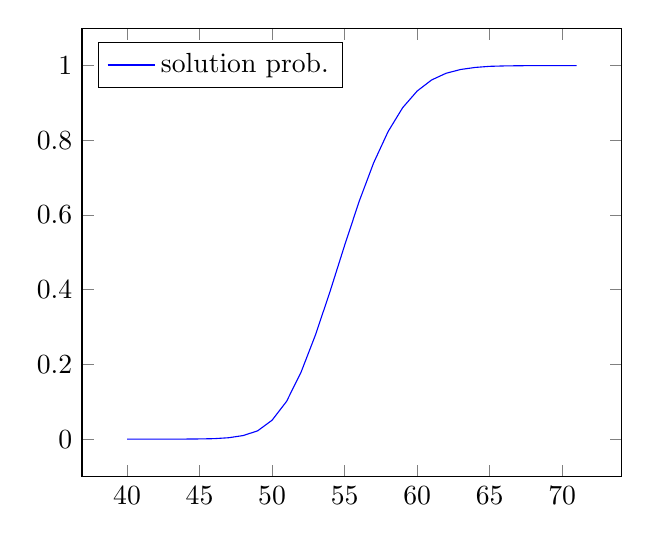
\begin{tikzpicture}
\begin{axis}[legend pos=north west]
\addplot[color=blue] coordinates {
(40,0) (41,0.00001) (42,0.00003) (43,0.0001) (44,0.00031) (45,0.00067)
(46,0.00141) (47,0.00385) (48,0.00967) (49,0.02222) (50,0.05076)
(51,0.10117) (52,0.17953) (53,0.27993) (54,0.39581) (55,0.51873)
(56,0.63614) (57,0.73955) (58,0.82352) (59,0.88719) (60,0.93182)
(61,0.9616) (62,0.97949) (63,0.98956) (64,0.99503) (65,0.99799)
(66,0.99907) (67,0.9996) (68,0.99989) (69,0.99997) (70,0.99998) (71,1) };
\addlegendentry{solution prob.}
\end{axis}
\end{tikzpicture}
\hspace{1cm}
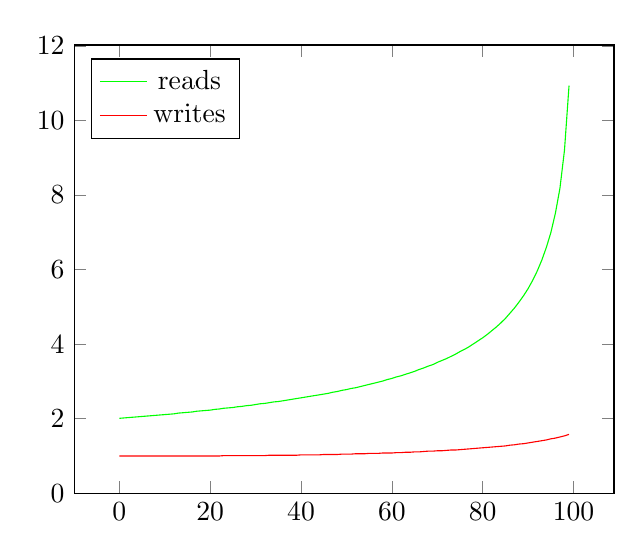
\begin{tikzpicture}
\begin{axis}[ymin=0, legend pos=north west]
\addplot[color=green] coordinates {
(0,2.01) (1,2.02) (2,2.03) (3,2.04) (4,2.05) (5,2.06) (6,2.07) (7,2.08) (8,2.09) (9,2.10) (10,2.11) (11,2.12) (12,2.13) (13,2.15) (14,2.16) (15,2.17) (16,2.18) (17,2.20) (18,2.21) (19,2.22) (20,2.23) (21,2.25) (22,2.26) (23,2.28) (24,2.29) (25,2.30) (26,2.32) (27,2.33) (28,2.35) (29,2.36) (30,2.38) (31,2.40) (32,2.41) (33,2.43) (34,2.45) (35,2.46) (36,2.48) (37,2.50) (38,2.52) (39,2.54) (40,2.56) (41,2.58) (42,2.60) (43,2.62) (44,2.64) (45,2.66) (46,2.68) (47,2.71) (48,2.73) (49,2.76) (50,2.78) (51,2.81) (52,2.83) (53,2.86) (54,2.89) (55,2.92) (56,2.95) (57,2.98) (58,3.01) (59,3.05) (60,3.08) (61,3.12) (62,3.15) (63,3.19) (64,3.23) (65,3.27) (66,3.32) (67,3.36) (68,3.41) (69,3.45) (70,3.51) (71,3.56) (72,3.61) (73,3.67) (74,3.73) (75,3.80) (76,3.86) (77,3.93) (78,4.01) (79,4.09) (80,4.17) (81,4.26) (82,4.36) (83,4.46) (84,4.57) (85,4.69) (86,4.83) (87,4.97) (88,5.13) (89,5.30) (90,5.49) (91,5.71) (92,5.96) (93,6.25) (94,6.59) (95,6.99) (96,7.51) (97,8.18) (98,9.20) (99,10.93) };
\addlegendentry{reads}
\addplot[color=red] coordinates {
(0,1.00) (1,1.00) (2,1.00) (3,1.00) (4,1.00) (5,1.00) (6,1.00) (7,1.00) (8,1.00) (9,1.00) (10,1.00) (11,1.00) (12,1.00) (13,1.00) (14,1.00) (15,1.00) (16,1.00) (17,1.00) (18,1.00) (19,1.00) (20,1.00) (21,1.00) (22,1.00) (23,1.01) (24,1.01) (25,1.01) (26,1.01) (27,1.01) (28,1.01) (29,1.01) (30,1.01) (31,1.01) (32,1.01) (33,1.02) (34,1.02) (35,1.02) (36,1.02) (37,1.02) (38,1.02) (39,1.02) (40,1.03) (41,1.03) (42,1.03) (43,1.03) (44,1.03) (45,1.04) (46,1.04) (47,1.04) (48,1.04) (49,1.05) (50,1.05) (51,1.05) (52,1.06) (53,1.06) (54,1.06) (55,1.07) (56,1.07) (57,1.07) (58,1.08) (59,1.08) (60,1.08) (61,1.09) (62,1.09) (63,1.10) (64,1.10) (65,1.11) (66,1.11) (67,1.12) (68,1.13) (69,1.13) (70,1.14) (71,1.14) (72,1.15) (73,1.16) (74,1.16) (75,1.17) (76,1.18) (77,1.19) (78,1.20) (79,1.21) (80,1.22) (81,1.23) (82,1.24) (83,1.25) (84,1.26) (85,1.27) (86,1.29) (87,1.30) (88,1.32) (89,1.33) (90,1.35) (91,1.37) (92,1.39) (93,1.41) (94,1.43) (95,1.46) (96,1.48) (97,1.51) (98,1.54) (99,1.58) };
\addlegendentry{writes}
\end{axis}
\end{tikzpicture}
\end{center}

\section{Difficulty control}
Relative easiness (the ratio $E/N$) determines a base level of difficulty,
which may suffice for applications where difficulty is to remain fixed.
The ratio $E/N=1$ is suitable when a practically guaranteed solution is desired,
For crypto currencies, where difficulty must scale in precisely
controlled manner across a huge range, adjusting easiness is not suitable.
The implementation default $E/N=1/2$ gives a solution probability of roughly $2.2\%$,
while the average number of cycles found increases slowly with size; from 2 at $2^{20}$
to 3 at $2^{30}$.
For further control, a diffculty target $0 < T < 2^{256}$ is introduced,
and we impose the additional constraint that the sha256 digest of the
cycle nonces in ascending order be less than $T$, thus
reducing the success probability by a factor $2^{256}/T$.

\section{Memory-hardness}
I conjecture that this problem doesn't allow for a time-memory trade-off. If
one were to store only a fraction $p$ of $V_0$ and $V_1$, then one would have
to reject a fraction $p^2$ of generated edges, drastically reducing the odds of
finding cycles for $p<1/\sqrt{2}$ (the reduction being exponential in cycle length).

\section{Parallelization}
The implementation allows the number of threads to be set with option {\tt -t}.
For $0\leq t < T$, thread $t$ processes all nonces $t \bmod T$.
Parallelization presents some algorithmic challenges. Paths from an edge's two endpoints
are not well-defined when other edge additions and path reversals are still in progress.
One example of such a path conflict is the check for duplicate edges yielding a false negative,
if in between checking the two endpoints, another thread reverses a path through those nodes.
Another is the addition of edges $(7,10)$ and $(3,15)$ in the example diagrams.
If these were to happen in parallel, then the path from $15$ will likely end at $5$ because
edge $(10 \rightarrow 5)$ hasn't been reversed yet.
As a result, $(3 \rightarrow 15)$ will be added, not realizing it creates a cyle.
Thus, in a parallel implementation, path following can no longer be assumed to terminate.
Instead of using a cycle detection algorithm such as~\cite{1980-brent-cycles}, our implementation
notices when the path length exceeds MAXPATHLEN (4096 by default),
and reports wether this is due to a path conflict.
The left plot below shows the average number of times that either of the two roots
for a nonce occurred a given number of nonces ago, showing that there are potentially
about $10T$ such conflicts.
Despite these conflicts, and the complete lack of synchronization between threads
(apart from a solution recording mutex),
the cuckoo array at any time represents some, possibly cyclic, directed cuckoo graph
on a subset of proccessed nonces.
On $2^{20}$ nodes, aborts happened 0.03\% of the time with 2 threads, 0.1\% with 4 threads, 0.27\% with
8 threars, and 0.2\% with 12 threads.
They overlooked 0.13\%, 0.31\%, 0.57\%, and 0.17\%, respectiverly, of the 42-cycles
found by the single-threaded runs.
Empirically then, path conflicts have negligable effect on multi-threaded performance.
The percentage of hashing to total runtime shows the same behaviour as in the single-threaded case,
with a dual Xeon X5670 machine spending only 5.5\% of wallclock time on hashing with $2^{28}$ nodes.

The right plot shows in green the speedup achieved by up to 40 threads on a system with two Intel Xeon
E5-2690 cpus, each which 10 hyperthreaded cores running at 3GHz.
Each datapoint represents 10 runs on $2^{30}$ nodes with headers "0" through "9".
Although the speedup is sublinear at 26 for 40 threads, it doesn't look like the memory interface
is saturated yet. Since we don't have access to more than 40 threads, we tried two alternative
approaches to see happens when the memory access frequency increases further,
In the first approach we reduce the number of rounds in the \hash function, shown in red and blue.
We checked with 10,000 test-runs on cuckoo125 that reducing the number of siphash rounds
has no noticeable effect on cycle length distribution.
In the second approach we precompute all the hashes, shown in orange.
This shows some sort of breakdown of the memory interface starting from 21 threads,
which is presumably where hyperthreading starts to kick in.
It is perhaps odd that such a hyperthreading transition is completely absent from the green line.
Since the hash precomputation showed a significant speedup, the implementation was changed
to make it the default. Reproducing the other curves requires compilation with -DPRESIP=0 for C or setting CuckooSolve.PRESIP=1 for java.

\begin{center}
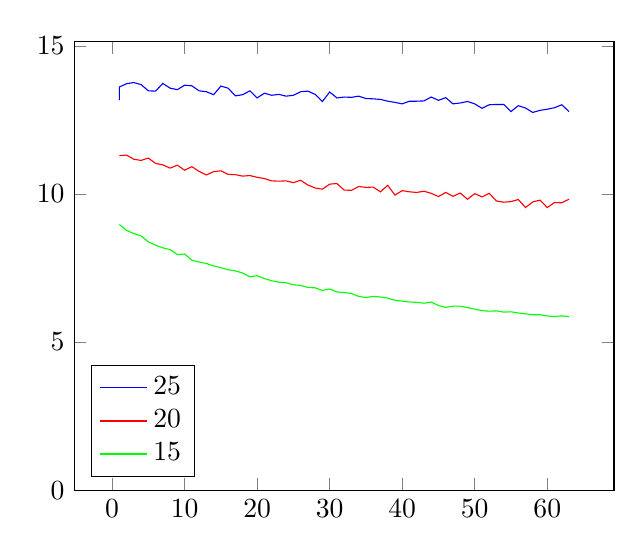
\begin{tikzpicture}
\begin{axis}[ymin=0, legend pos=south west]
\addplot[color=blue] coordinates {
(1,13.17)(1,13.61) (2,13.72) (3,13.76) (4,13.69) (5,13.48) (6,13.47) (7,13.73) (8,13.57) (9,13.52) (10,13.67) (11,13.65) (12,13.48) (13,13.45) (14,13.35) (15,13.64) (16,13.57) (17,13.31) (18,13.35) (19,13.48) (20,13.24) (21,13.40) (22,13.33) (23,13.36) (24,13.30) (25,13.33) (26,13.45) (27,13.47) (28,13.36) (29,13.12) (30,13.44) (31,13.24) (32,13.27) (33,13.26) (34,13.30) (35,13.22) (36,13.21) (37,13.19) (38,13.13) (39,13.09) (40,13.04) (41,13.13) (42,13.13) (43,13.14) (44,13.27) (45,13.16) (46,13.25) (47,13.04) (48,13.07) (49,13.12) (50,13.04) (51,12.89) (52,13.01) (53,13.02) (54,13.02) (55,12.78) (56,12.98) (57,12.90) (58,12.75) (59,12.82) (60,12.86) (61,12.91) (62,13.01) (63,12.78) };
\addlegendentry{25}
\addplot[color=red] coordinates {
(1,11.29) (2,11.31) (3,11.17) (4,11.13) (5,11.21) (6,11.03) (7,10.98) (8,10.87) (9,10.97) (10,10.80) (11,10.92) (12,10.76) (13,10.64) (14,10.75) (15,10.78) (16,10.66) (17,10.65) (18,10.60) (19,10.62) (20,10.56) (21,10.52) (22,10.44) (23,10.43) (24,10.44) (25,10.38) (26,10.46) (27,10.30) (28,10.20) (29,10.16) (30,10.33) (31,10.35) (32,10.13) (33,10.12) (34,10.25) (35,10.22) (36,10.23) (37,10.07) (38,10.29) (39, 9.96) (40,10.11) (41,10.07) (42,10.05) (43,10.09) (44,10.02) (45, 9.91) (46,10.05) (47, 9.92) (48,10.03) (49, 9.82) (50,10.01) (51, 9.90) (52,10.02) (53, 9.76) (54, 9.72) (55, 9.74) (56, 9.81) (57, 9.54) (58, 9.73) (59, 9.79) (60, 9.54) (61, 9.71) (62, 9.70) (63, 9.82) };
\addlegendentry{20}
\addplot[color=green] coordinates {
(1, 8.97) (2, 8.77) (3, 8.66) (4, 8.58) (5, 8.38) (6, 8.27) (7, 8.18) (8, 8.12) (9, 7.95) (10, 7.97) (11, 7.76) (12, 7.70) (13, 7.65) (14, 7.57) (15, 7.51) (16, 7.44) (17, 7.40) (18, 7.33) (19, 7.20) (20, 7.24) (21, 7.14) (22, 7.07) (23, 7.02) (24, 7.00) (25, 6.93) (26, 6.91) (27, 6.84) (28, 6.83) (29, 6.74) (30, 6.79) (31, 6.69) (32, 6.67) (33, 6.64) (34, 6.54) (35, 6.50) (36, 6.54) (37, 6.52) (38, 6.48) (39, 6.41) (40, 6.38) (41, 6.35) (42, 6.34) (43, 6.31) (44, 6.35) (45, 6.23) (46, 6.17) (47, 6.21) (48, 6.21) (49, 6.16) (50, 6.11) (51, 6.06) (52, 6.04) (53, 6.05) (54, 6.01) (55, 6.02) (56, 5.98) (57, 5.95) (58, 5.92) (59, 5.92) (60, 5.88) (61, 5.86) (62, 5.88) (63, 5.86) };
\addlegendentry{15}
\end{axis}
\end{tikzpicture}\hspace{1cm}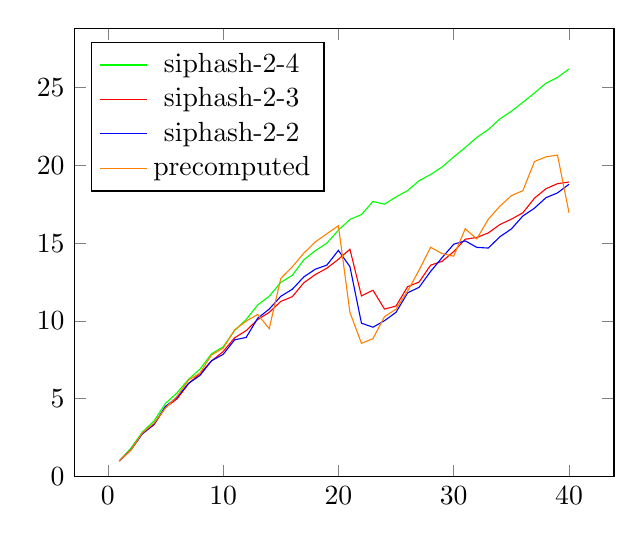
\begin{tikzpicture}
\begin{axis}[ymin=0, legend pos=north west]
\addplot [color=green] coordinates {
(1,1.000) (2,1.820) (3,2.858) (4,3.560) (5,4.700) 
(6,5.374) (7,6.249) (8,6.904) (9,7.895) (10,8.332) 
(11,9.382) (12,10.091) (13,11.025) (14,11.586) (15,12.477) 
(16,12.929) (17,13.928) (18,14.517) (19,14.998) (20,15.832) 
(21,16.521) (22,16.834) (23,17.677) (24,17.501) (25,17.971) 
(26,18.374) (27,19.012) (28,19.412) (29,19.894) (30,20.537) 
(31,21.143) (32,21.790) (33,22.298) (34,22.979) (35,23.469) 
(36,24.050) (37,24.642) (38,25.279) (39,25.647) (40,26.190) 
};
\addlegendentry{siphash-2-4}
\addplot [color=red] coordinates {
(1,1.000) (2,1.700) (3,2.757) (4,3.322) (5,4.438) 
(6,4.986) (7,5.961) (8,6.628) (9,7.426) (10,8.029) 
(11,8.914) (12,9.377) (13,10.090) (14,10.549) (15,11.252) 
(16,11.555) (17,12.451) (18,12.979) (19,13.388) (20,13.961) 
(21,14.604) (22,11.605) (23,11.971) (24,10.761) (25,10.958) 
(26,12.200) (27,12.501) (28,13.581) (29,13.831) (30,14.457) 
(31,15.251) (32,15.361) (33,15.654) (34,16.192) (35,16.538) 
(36,16.950) (37,17.885) (38,18.493) (39,18.822) (40,18.928) 
};
\addlegendentry{siphash-2-3}
% \addplot [color=orange] coordinates {
% (1,1.000) (2,1.713) (3,2.720) (4,3.319) (5,4.405) 
% (6,4.984) (7,5.847) (8,6.324) (9,7.350) (10,7.817) 
% (11,8.658) (12,9.181) (13,10.007) (14,10.511) (15,11.325) 
% (16,11.785) (17,12.594) (18,13.050) (19,13.382) (20,14.081) 
% (21,13.179) (22,9.398) (23,8.713) (24,9.777) (25,10.284) 
% (26,11.384) (27,11.876) (28,12.824) (29,13.556) (30,14.216) 
% (31,14.792) (32,13.778) (33,14.162) (34,14.759) (35,15.382) 
% (36,15.894) (37,16.621) (38,17.198) (39,17.636) (40,17.950) 
% };
% \addlegendentry{siphash-1-1}
\addplot [color=blue] coordinates {
(1,1.000) (2,1.721) (3,2.752) (4,3.360) (5,4.503) 
(6,5.074) (7,5.989) (8,6.499) (9,7.445) (10,7.847) 
(11,8.786) (12,8.938) (13,10.174) (14,10.761) (15,11.579) 
(16,12.036) (17,12.826) (18,13.326) (19,13.588) (20,14.531) 
(21,13.487) (22,9.856) (23,9.595) (24,10.016) (25,10.558) 
(26,11.805) (27,12.161) (28,13.184) (29,14.075) (30,14.927) 
(31,15.145) (32,14.726) (33,14.682) (34,15.405) (35,15.910) 
(36,16.746) (37,17.242) (38,17.918) (39,18.225) (40,18.780) 
};
\addlegendentry{siphash-2-2}
% \addplot [color=orange] coordinates {
% (1,1.000) (2,1.716) (3,2.758) (4,3.366) (5,4.488) 
% (6,5.020) (7,6.050) (8,6.479) (9,7.436) (10,7.968) 
% (11,8.790) (12,9.312) (13,10.268) (14,10.688) (15,11.589) 
% (16,11.937) (17,12.835) (18,13.374) (19,13.694) (20,14.393) 
% (21,13.419) (22,9.770) (23,9.147) (24,10.018) (25,10.541) 
% (26,11.660) (27,11.983) (28,13.337) (29,13.860) (30,14.887) 
% (31,15.214) (32,14.130) (33,14.371) (34,15.349) (35,15.692) 
% (36,16.242) (37,16.981) (38,17.522) (39,17.945) (40,18.598) 
% };
% \addlegendentry{siphash-1-2}
\addplot [color=orange] coordinates {
(1,1.000) (2,1.712) (3,2.805) (4,3.428) (5,4.396) 
(6,5.152) (7,6.194) (8,6.655) (9,7.820) (10,8.245) 
(11,9.424) (12,9.986) (13,10.417) (14,9.504) (15,12.722) 
(16,13.477) (17,14.356) (18,15.078) (19,15.602) (20,16.117) 
(21,10.547) (22,8.559) (23,8.864) (24,10.274) (25,10.760) 
(26,11.915) (27,13.263) (28,14.735) (29,14.326) (30,14.162) 
(31,15.923) (32,15.268) (33,16.536) (34,17.369) (35,18.049) 
(36,18.371) (37,20.241) (38,20.545) (39,20.656) (40,16.951) 
};
\addlegendentry{precomputed}
\end{axis}
\end{tikzpicture}
\end{center}

\section{Choice of cycle length}
Extremely small cycle lengths risk the feasability of alternative datastructures that
are more memory-efficient. For example, for $L=2$ the problem reduces to finding a birthday collision
as in the Momentum proof-of-work.
It is conceivable however that the Cuckoo representation is already optimal for $L=4$.
Such small values still harm the TMTO resistance though, as mentioned in the previous paragraph,
and may reduce parallelization resistance.
In order to keep proof size manageable, the cycle length should not be too large either.
We consider 20-64 to be a healthy range, which averages to 42.
The plot below shows the distribution of cycle lengths found for sizes $2^{10},2^{15},2^{20},2^{25}$,
as determined from 100000,100000,10000, and 10000 runs respectively. The tails of the distributions
beyond $L=100$ are not shown. For reference, the longest cycle found was of length 2120.

\begin{center}
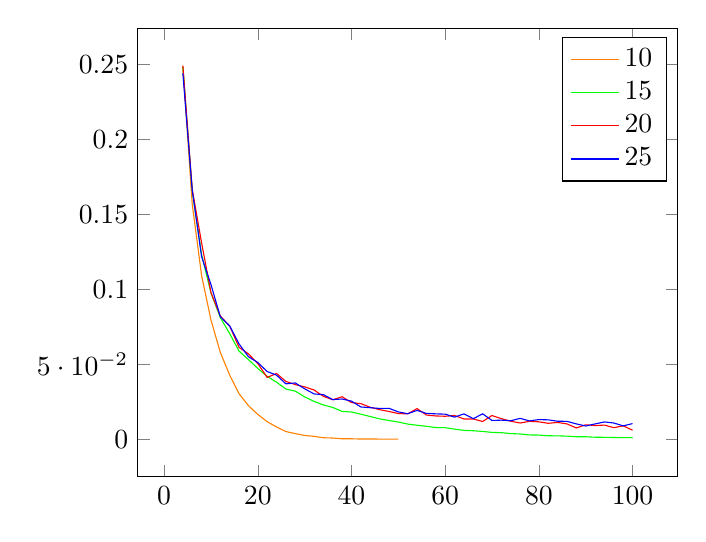
\begin{tikzpicture}
\begin{axis}
\addplot[color=orange] coordinates {
(4,0.24862) (6,0.15673) (8,0.10907) (10,0.07952) (12,0.05783) (14,0.04269) (16,0.0303)
(18,0.02237) (20,0.01653) (22,0.01168) (24,0.00815) (26,0.00511) (28,0.00374) (30,0.00251)
(32,0.00191) (34,0.00098) (36,0.00079) (38,0.00029) (40,0.0003) (42,0.00011) (44,0.00018)
(46,8e-05) (48,2e-05) (50,3e-05) };
\addlegendentry{10}
\addplot[color=green] coordinates {
(4,0.24822) (6,0.16551) (8,0.12317) (10,0.09749) (12,0.08105) (14,0.07036) (16,0.05871) (18,0.05308)
(20,0.04717) (22,0.04189) (24,0.03801) (26,0.03342) (28,0.03205) (30,0.02822) (32,0.02521)
(34,0.02282) (36,0.0212) (38,0.01852) (40,0.01814) (42,0.01668) (44,0.01511) (46,0.01356)
(48,0.01246) (50,0.01145) (52,0.0101) (54,0.0093) (56,0.00861) (58,0.00778) (60,0.00768)
(62,0.00672) (64,0.00589) (66,0.00565) (68,0.00517) (70,0.00455) (72,0.00435) (74,0.00375)
(76,0.00348) (78,0.00286) (80,0.00276) (82,0.0023) (84,0.00224) (86,0.00204) (88,0.00165)
(90,0.00164) (92,0.00134) (94,0.00126) (96,0.00114) (98,0.00103) (100,0.00101) };
\addlegendentry{15}
\addplot[color=red] coordinates {
(4,0.249) (6,0.1666) (8,0.1309) (10,0.0977) (12,0.0821) (14,0.0754) (16,0.0612) (18,0.0569)
(20,0.0504) (22,0.0412) (24,0.0438) (26,0.0385) (28,0.0364) (30,0.0349) (32,0.0328) (34,0.0286)
(36,0.0263) (38,0.0283) (40,0.0244) (42,0.0237) (44,0.0213) (46,0.0197) (48,0.0185) (50,0.0171)
(52,0.0169) (54,0.0204) (56,0.0161) (58,0.0155) (60,0.0153) (62,0.0158) (64,0.0135) (66,0.0135)
(68,0.0118) (70,0.0158) (72,0.0137) (74,0.012) (76,0.0108) (78,0.0119) (80,0.0116) (82,0.0106)
(84,0.0112) (86,0.0102) (88,0.0075) (90,0.0096) (92,0.0091) (94,0.0094) (96,0.0077) (98,0.0089)
(100,0.006) };
\addlegendentry{20}
\addplot[color=blue] coordinates {
(4,0.2439) (6,0.1661) (8,0.1216) (10,0.1031) (12,0.0816) (14,0.0755) (16,0.0635) (18,0.055) (20,0.0511) (22,0.0451) (24,0.0427) (26,0.0369) (28,0.0375) (30,0.0336) (32,0.0302) (34,0.0297) (36,0.0264) (38,0.0268) (40,0.0254) (42,0.0215) (44,0.021) (46,0.0205) (48,0.0206) (50,0.0182) (52,0.017) (54,0.0192) (56,0.0172) (58,0.0169) (60,0.0167) (62,0.0147) (64,0.0169) (66,0.0137) (68,0.0169) (70,0.0125) (72,0.0127) (74,0.0123) (76,0.0139) (78,0.0122) (80,0.0131) (82,0.0129) (84,0.012) (86,0.0119) (88,0.0102) (90,0.0088) (92,0.0102) (94,0.0115) (96,0.0108) (98,0.0089) (100,0.0104) };
\addlegendentry{25}
\end{axis}
\end{tikzpicture}
\end{center}

\section{Choice of memory size}
The memory requirement should exceed that of the largest available
single-chip memory to enforce off-chip latencies. It should also be a
significant fraction of the typical memory of a botnet computer,
With a significant risk of sending machines into swap-hell and
likely alerting its owner, botnet operators will refrain from deploying
Cuckoo Cycle, prefering other proof-of-work schemes whose smaller memory
footprint allows them to stay under the radar.
With memory sizes doubling roughly every 18 months, 16GB will become
commonplace in a few years.
While the current algorithm can accomodate up to $N=2^{33}-2$ nodes
(32GB) by separately keeping track of which partition a vertex is in,
a different idea is needed to scale beyond that.
To that end, we propose to use $K$-partite graphs with edges only between
partition $k$ and partition $(k+1) \bmod K$, where $k$ is fed into the hash
function along with the header and nonce. With each partition consisting of
at most $2^{31}-1$ nodes, the most significant bit is then available to
distinguish edges to the two neighbouring partitions.
Setting the size of partition 0 to be relatively prime to $2(K-1)$,
and making each successive partition smaller by 2,
ensures that neighbouring partition sizes are relatively prime.

\section{Conclusion}
Cuckoo Cycle is an elegant proof-of-work design emphasizing memory latency
over computation.  This promotes investment in low-power general purpose
hardware (RAM) rather than investment in single purpose hardware coupled with
high operational costs, making mining more sustainable.  More research is
needed to determine the limits of parallelizability.

\bibliographystyle{IEEEtran}
\bibliography{cuckoo}

\lstset{language=C,basicstyle=\footnotesize}
\section{Appendix A: cuckoo.h}
\lstinputlisting{cuckoo.h}

\section{Appendix B: cuckoo\_miner.h}
\lstinputlisting{cuckoo_miner.h}

\section{Appendix C: cuckoo\_miner.c}
\lstinputlisting{cuckoo_miner.c}

\end{document}  
